% !TEX root = main.tex
\section{Discussion\label{sec:6_disc}}

There are various aspects of the results above that warrant further discussion. First, we will discuss the likelihood that conclusions based on these results can be generalized to a broad range of physical dislocation systems. Secondly, we will attempt to speculate as to why the global distributions found were approximately Cauchy in shape and why the maximum entropy approximation poorly described the shape of the distributions. Following this, we briefly discuss the bearing of the findings on the closure of the evolution hierarchy. Lastly, we discuss a more exotic use case for the fluctuation distributions just reported---a possible implication for continuum treatments of dislocation reaction processes.

\subsection{Applicability of results}\label{applicability-of-results}
The main results of the calculations performed can be summarized as follows. For very small coarse-graining lengths (\(L <\) 200 nm or \(L < L_{\rho}/4\)), the dislocation density is highly polarized (\(\beta_{1} > 0.9\)). This means that the continuum system can be treated analogously to a discrete density field. For intermediate coarse-graining lengths where the polarization deviates substantially from unity (\(1/4 < L/L_\rho < 2/3)\ \)closure of the density hierarchy may be performed appropriately by means of line bundle approximations which assume the characteristic sequence is roughly geometric. For coarse-graining lengths approaching the average dislocation spacing, neither of the candidate closure relations (line bundle or maximum entropy) was appropriate.

For what types of dislocation systems do these findings hold? The systems considered were sparse: the average spacing between dislocations of like slip system in these systems is on the order of \SI{2}{\micro\metre}. As strains progress, the dislocation spacing decreases. In more dense systems, it is unclear whether the angular distributions would be more dependent on the absolute coarse-graining length or the ratio of the coarse-graining length to the average spacing. On the one hand, it would seem that the length relative to the spacing should determine the orientation statistics. However, there also exist absolute length scales associated with physical dislocations. Certain dislocation properties may also affect the orientation statistics, such as reaction lengths or the distance on which oppositely signed dislocations annihilate (often taken to be on the order of 50 nm \cite{Lin2021}). To answer the question of this distinction, one would need discrete simulations with a settled treatment of dislocation reactions and densities on the order of \SI{1000}{\micro\metre^{-2}}. At the moment, this is simply not feasible. In principle, these orientation statistics could be accessible to experiment (cf. dark field x-ray microscopy\cite{simonsDarkfieldXrayMicroscopy2015,poulsenGeometricalopticsFormalismModel2021,borgiSimulationsDislocationContrast2024}) by means of the strain distributions in small crystalline regions, but again, this lies beyond the reaches of the current state-of-the-art. In the meantime, the ambiguity between absolute and relative distances cannot be satisfactorily resolved and we encourage the use of the above results in either sense.

\subsection{The Cauchy shape of the fluctuation distribution}
One of our major findings in the present work concerns the shape of the orientation fluctuation distributions. The maximum entropy assumption results in von Mises-type distributions (generalizations of the Gaussian distribution on a circular domain with higher order moments constrained), while the distributions observed were better represented by (wrapped) Cauchy distributions. This difference in shape resulted in the relatively poor predictive ability for the maximum entropy relations in closing the hierarchy of kinematic variables. The question naturally arises as to why the distribution might be Cauchy instead of maximum entropy in shape. Any answer given to this question will obviously be heuristic and \emph{a posteriori}, but let us attempt one nonetheless. Two possibilities present themselves: 1) the orientation fluctuations are a ratio of Gaussian random variables~\cite{mardiaStatisticsDirectionalData1975} or 2) there are two independent Gaussian processes with different second moments are contributing simultaneously to produce orientation fluctuations~\cite{baileyEmergenceWrappedCauchy2021}. We will focus on the former. If the likelihood of a fluctuation angle is related to its ratio to a representative angular scale which is also a random variable, the Cauchy shape may be produced. The natural candidate for this is curvature, which determines the spatial strength of changes in line orientation. Considering a segment of uniform curvature passing through a volume (a circular arc). The orientations would be uniformly distributed on an interval \(\delta \in \left\lbrack - |\kappa l|/2,|\kappa l|/2 \right\rbrack\) where \(\kappa\) is the curvature of the arc and \(l\) is the length of the arc; the term \(|\kappa l|\) is properly related to the local curvature density \(q\). If the likelihood of a fluctuation is related to the weight it contributes to a point relative to the curvature density of the segment and both are random variables, a Cauchy shape could result. Another line of reasoning might proceed from Gibbs-type energy penalization of perturbations of dislocation lines via their change to the arc-length of the dislocation line, which would also depend inversely on curvature.

Nonetheless, any additional information regarding the shape of the distribution cuts against the maximum entropy problem approach. The maximum entropy approach assumes that the only knowledge we have of the system, qualitative or quantitative, is the first \(n\) moments of the distribution. Prior knowledge of the orientation fluctuation as a rational process would then have to be taken into account as an additional constraint in the entropy maximization process. Thus, the strong leaning of the distributions towards a Cauchy-like shape points to at least a qualitative `hidden variable'; that is, something we \emph{ought} to know about the orientation fluctuation process before simply leaping into the entropy maximization operation. Even at the large coarse-graining lengths the maximum entropy approach was designed to treat, we see it break down. This is presumably due to some important hidden information regarding the process that is not captured simply by the first few moments. Especially notable was the poor performance of the first order maximum entropy closure due to a quickly decaying term which was not present in the data. I would guess that this poor agreement was what led to the generally poor performance of the first order closure in the initial dynamical benchmarking study of the maximum entropy closure~\cite{Monavari2016}.

\subsection{Implications for the evolution equations}
The different length scale regimes noted above warrant different treatments of the dislocation dynamics. Regardless of which regime is being considered, all of these treatments amount to a closure of the density hierarchy at some fixed order. However, inspection of the evolution equations \cref{eq:11_reducedEvolution} reveals that the auxiliary curvature tensor hierarchy also needs to be similarly closed. In the case that the curvature is homogeneous in the orientation coordinate, the auxiliary curvature tensors can be expressed as:
\begin{subequations}
\begin{align}
\mathbf{Q}^{(n)}(\boldsymbol{r}) &= \kappa\left( \boldsymbol{r} \right)\rho\left( \boldsymbol{r} \right)\int_{S^{1}}^{}{f_{\boldsymbol{r}}(\varphi)\boldsymbol{p}^{\otimes2}(\varphi)\boldsymbol{l}^{\otimes n - 2}(\varphi)d\varphi}\\    
&= q\left( \boldsymbol{r} \right)\ \text{sym}\left\lbrack \widehat{\boldsymbol{n}}\times\left\langle \boldsymbol{l}^{\otimes n} \right\rangle_{\boldsymbol{r}} \times \widehat{\boldsymbol{n}} \right\rbrack
\end{align}
\end{subequations}
Still, this requires fixing the curvature \(\kappa\boldsymbol{(r)}\). It has been shown~\cite{Sedlacek2010,Hochrainer2010,zhangContinuumDislocationDynamics2025} that in the purely polarized state, the curvature is given by:
\begin{equation}
\kappa\left( \boldsymbol{r} \right) \coloneqq {\overline{\boldsymbol{l}}}_{\boldsymbol{r}}\cdot\nabla{\overline{\varphi}}_{\boldsymbol{r}}
\end{equation}
or in a coordinate-independent form
\begin{equation}
\kappa\left( \boldsymbol{r} \right)=\left( \hat{\boldsymbol{n}}\times\nabla \right)\cdot{\overline{\boldsymbol{l}}}_{\boldsymbol{r}}
\end{equation}
This can be seen by expanding the time derivative of the vector magnitude of the first order evolution equation {[}\cref{eq:11_reducedEvolution}{]} and comparing it to the zeroth order equation. This expression also holds for systems where the polarization gradients are small.

Although we have seen that there are highly polarized regimes of dislocation dynamics (where \(L < 200\) nm), the more significant range is that where the polarization is non-negligible but the line bundle closure is still valid (\(L < 2L_{\rho}/3\)). In this case, it would be worthwhile to express the curvature in terms of its completely polarized contribution {[}Eq. (21){]} as well as some additional curvature source tied to the `statistically stored' portion of the density (\(\epsilon(\boldsymbol{r)} = 1 - \beta_{1}(\boldsymbol{r})\)). While the closure of the density hierarchy at small scales has been demonstrated in the present work, a definitive linking of the discrete scale to the macroscopic case (where curvature must be treated as a dynamic quantity) would involve fixing the curvature in terms of density-based quantities (as is done at large coarse-graining lengths in~\cite{zhangContinuumDislocationDynamics2025}).

Assuming this discrete expression for the curvature, one finds that in systems with high or constant polarization, the discrete curl-type transport equation is sufficient to describe the system. This treatment we have been referring to as vector density dislocation dynamics\cite{Anderson2022}. Nonetheless, the line bundle assumption still has implications even for the curl transport equation. When one moves to a consideration of kinetics, the velocity is dependent on the line direction by means of the Peach Koehler force:
\begin{equation}
\boldsymbol{v}=M\left( \boldsymbol{b} \cdot \boldsymbol{\sigma}\left( \boldsymbol{r} \right) \right)\times \boldsymbol{l}
\end{equation}
Upon averaging the transport equation, the second-order alignment tensor thus appears:
\begin{subequations}
\begin{align}
    \partial_{t}\boldsymbol{\rho}&=\nabla\times\left\langle \boldsymbol{v}\times\rho\boldsymbol{l} \right\rangle\\
    &= M\nabla \times \left\langle \left( \left( \boldsymbol{b} \cdot \boldsymbol{\sigma} \right)\times\boldsymbol{l} \right)\times \boldsymbol{l} \right\rangle\\
    &=M\ \nabla \times \left\langle \boldsymbol{b}\cdot \boldsymbol{\sigma} \cdot \left( \boldsymbol{l}^{\otimes2}-\mathbb{ I} \right)\rho \right\rangle
\end{align}
\end{subequations}
Averages of this form are the motivation for the more general form of the line bundle assumption utilized in the appendix. This version allows a single factor of \(\boldsymbol{l}\) to be factored out of such averages, resulting in a kinetic equation expressible in terms of the vector density and a suitable correlation function. For a more detailed treatment of this question of kinetics, we refer the reader to a previous work\cite{andersonDislocationCorrelationsContinuum2024}.

Beyond the quasi-discrete regime of high polarization, the present findings anticipate new treatments of continuum dislocation dynamics at intermediate length scales. Closing the evolution equations at second order while utilizing the discrete curvature expression is a new possibility. Corrections to the discrete evolution equation based on weak gradients in the polarization field may also be considered. We hope that the present work inspires new hybrid approaches blending the quasi-discrete vector density transport and the hopelessly general higher-order density transport. It is our opinion that progress toward an understanding of fundamental deformation phenomena at small scales---such as fatigue, the onset of dislocation patterning, and even crack dynamics---will come from hybrid approaches in the intermediate regime where the line bundle assumption holds with non-trivial polarizations. In this spirit, we next turn our attention to how the present results would inform the physics of dislocation interactions in such an intermediate regime.

\subsection{Implications for continuous dislocation reactions}
{Dislocation reactions result in interchange of density between slip systems, resulting in the coupling of dislocation evolution equations in a manner analogous to reaction-diffusion methods:} 
\begin{align}
\dot{\boldsymbol{\rho}}^{[\alpha]}_j=&\dot{\boldsymbol{\rho}}^{[\alpha]}_\text{glide}  +\dot{\boldsymbol{\rho}}^{[\alpha],\text{cs}} +\dot{\boldsymbol{\rho}}^{[\alpha],\text{gj}} -\dot{\boldsymbol{\rho}}^{[\alpha],\text{sj}}\\
(\dot{\boldsymbol{\rho}}^{[\alpha],\text{cs}})_j =& \rho^{[\alpha']}_j\dot{r}^{[\alpha',cs]}\left(\bar{\psi}^{[\alpha']},\sigma_{ij}(\boldsymbol{r})\right) \nonumber \\&- \rho^{[\alpha]}_j\dot{r}^{[\alpha,cs]}\left(\bar{\psi}^{[\alpha]},\sigma_{ij}(\boldsymbol{r})\right)\\
(\dot{\boldsymbol{\rho}}^{[\alpha],\text{gj}})_k =& \sum_{\beta,\gamma} \rho^{[\beta]}_i\rho^{[\gamma]}_j \dot{r}^{[\beta,\gamma\to\alpha, \text{gj}]}_{ij}(\bar\psi^{[\beta]},\bar\psi^{[\gamma]}) \nonumber \\
&- \rho^{[\alpha]}_i\sum_\beta\dot r^{[\alpha,\beta\to \gamma, \text{gj}]}_{ij}(\bar\psi^{[\alpha]},\bar\psi^{[\beta]})\\
(\dot{\boldsymbol{\rho}}^{[\alpha],\text{sj}})_k =&  \rho^{[\alpha]}_i\sum_{\beta}\dot \rho_j^{[\beta]}r^{[\alpha,\beta\to s]}_{ijk}(\bar\psi^{[\alpha]},\bar\psi^{[\beta]})
\end{align}
where $\dot{\boldsymbol{\rho}}_\text{slip}$ is the density evolution due to dislocation glide that we have been thus far discussing, and $\dot{\boldsymbol{\rho}}^{[\alpha],\text{cs}} ,\dot{\boldsymbol{\rho}}^{[\alpha],\text{gj}},\dot{\boldsymbol{\rho}}^{[\alpha],\text{sj}}$ are the net production (positive) or loss (negative) of dislocation density due to various reactions (cross-slip, glissile junction, and sessile junction). The rates of these reactions $\dot r$ generally vary based on the type of reaction and are dependent on the orientation of the reacting systems' density vectors with respect to the slip plane dihedral $(\bar{\psi})$. In the case of cross slip, each system $\alpha$ has only one cross-slip system $\alpha'$, and the rate is additionally dependent on the local stress state. The interested reader is referred to \cite{Vivekanandan2021} for a more detailed discussion of these rates.

In discrete dislocation systems, there are several modes by which dislocations might react with each other to form junction segments. This process begins with a crossed state, where two dislocations on separate slip planes intersect. These two dislocations are described by their respective angles \(\psi_{1},\psi_{2}\) with respect to the dihedral formed by the two glide planes. In certain regions of the two-dimensional orientation space, this crossed state is unstable: the formation of a junction segment along the dihedral would lower the elastic energy of the system. Thus, the reaction is considered to be a deterministic process:  if the energy criterion is satisfied, the crossed state always forms a junction; if not, the dislocations glide past each other and form a jog. The deterministic reaction maps (using the energy criterion of~\cite{Lin2020,madecNatureAttractiveDislocation2002}) are shown in \cref{fig:reactionmaps}a-c: white denotes the formation of a junction while black denotes jog formation. We consider these maps to be a function taking unit value in the reacting region and null in the complement:
\begin{equation}
\dot r=1_{\Delta E < 0}\left( \psi_{1},\psi_{2} \right) = 
\begin{dcases}
1 & \text{for junction formation},  \\
0 & \text{otherwise}.
\end{dcases} 
\end{equation}
In the continuum system, we do not have access to the direction of each individual dislocation at a given point. We do, however, have access to the average direction of dislocations at a given point \({\overline{\psi}}_{1},{\overline{\psi}}_{2}\). Additionally, we know the likelihood of fluctuations from that direction in an average sense. {Additionally, the relatively small size of these angular fluctuations allows the preservation of analogous behavior to the discrete system. As a result, the fluctuation information can be used to determine the likelihood of a dislocation reaction for a given pair of average directions:}
\begin{widetext}
\begin{equation}
\dot{r} =P_{j}^{(L)}\left( {\overline{\psi}}_{1},{\overline{\psi}}_{2} \right) = \int_{0}^{2\pi}{d\delta_{1}\int_{0}^{2\pi}{d\delta_{2}}f^{(L)}\left( \delta_{1} \right)f^{(L)}\left( \delta_{2} \right)1_{\Delta E < 0}\left( \overline{\psi}_{1} + \delta_{1},{\overline{\psi}}_{2} + \delta_{2} \right)}.
\end{equation}
\end{widetext}
\begin{figure*}
    \centering
    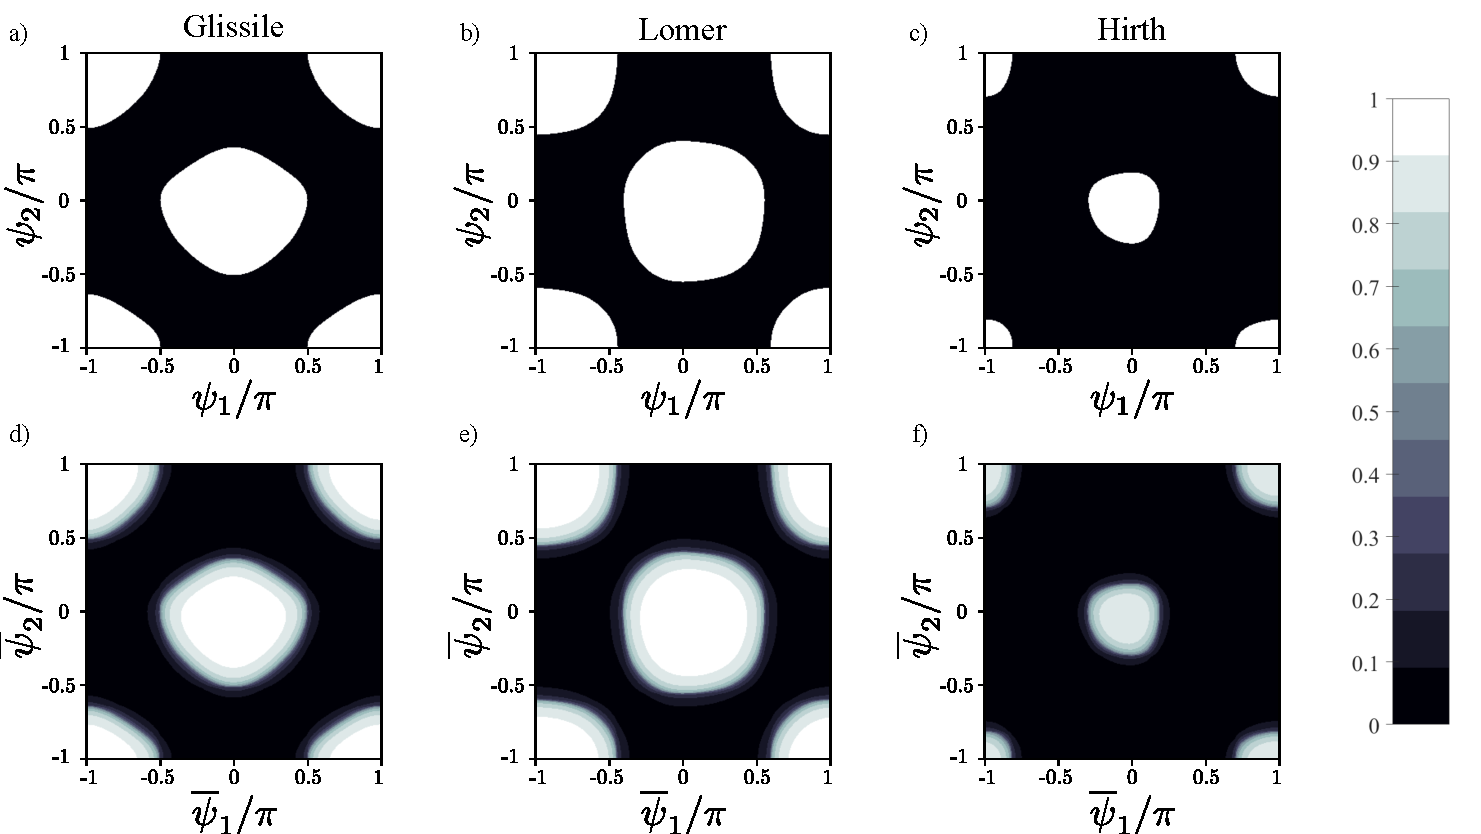
\includegraphics[width=0.8\linewidth]{Images/fig6.pdf}
    \caption{Discrete and Continuum reaction maps. The pairs of angles (measured with respect to the dihedral direction) which result in the three junction types---glissile junction, Lomer lock, Hirth lock---for discrete dislocation segments are shown in (a-c), respectively. The corresponding maps for continuum dislocation density vectors (d-f) give the likelihood that discrete segments in the collection fall within the reaction region. The orientation fluctuation distribution functions used to obtain the continuum reaction maps were calculated using a 97 nm coarse-graining length.}
    \label{fig:reactionmaps}
\end{figure*}
This is simply the convolution of the discrete reaction map with the joint fluctuation distribution (the two fluctuation processes are independent\footnote{Similar analysis to section 4 was performed to calculate the joint distributions for dislocations within a cutoff radius; no deviation from the independent joint distribution was found even for small cutoff radii.}). The resulting continuous reaction maps are shown in \cref{fig:reactionmaps}d-f.

One of the central results of this work was the observation that local fluctuations in dislocation orientation were of finite strength and that
their distribution could be measured. The implication is that at any continuum scale, orientation-dependent processes must consider this uncertainty in the precise directions of the underlying dislocations. This holds not only for deterministic processes such as the reactions just considered, but also for probabilistic processes such as cross-slip~\cite{vivekanandanDataDrivenApproach2023}. This example serves to show that the implications of orientation fluctuations reach beyond the closure of the evolution hierarchy.

\section{Conclusion}
In the present work, we have put forward a treatment of the average strength of orientation fluctuations in a spatially coarse-grained continuum treatment of dislocations. A key feature of this analysis was the fluctuation distribution function which describes the distribution of small deviations from the local average dislocation orientation. These fluctuations are closely related to the coarse-graining length, as it controls the size of the region wherein dislocations are treated collectively. In addition to the local fluctuation distribution, the total volume average of this distribution---the global fluctuation distribution---was put forward to explicitly analyze the dependence of local orientations on coarse-graining length in an average sense.

The importance of the fluctuation distributions governing deviations from the local average orientation on the transport was discussed in the context of the higher-order treatment of the evolution of dislocations distributed across orientation~\cite{Hochrainer2015}. A key concept in this treatment is the characteristic sequence of the distribution (its Fourier coefficients). A reduced form of the higher-order transport is given by closing this sequence at low order. Two such closure approximations were considered. First, the line bundle approximation---novel to the present work---was derived from assuming neighboring entries in the characteristic sequence are geometric, a trait we refer to as Cauchy-like. For comparison, we also evaluated the maximum entropy approximation due to Monavari et al.~\cite{Monavari2016}. It was also shown that the validity of the closure approximations at a given coarse-graining length could be evaluated from the global fluctuation distribution.

Measurements of the global fluctuation distribution were performed using discrete dislocation dynamics simulations. These simulations were analyzed at various coarse-graining lengths. The resulting distributions were approximately Cauchy in shape, having an additional spike at zero fluctuation due to the discretization of the dislocation segments. At small coarse-graining lengths, this distribution was sharply concentrated at zero fluctuations, with the distribution broadening at larger coarse-graining lengths. An analysis of the characteristic sequence of the measured distributions found that very short coarse-graining lengths (\(L < 200\ nm\ \)or 1/4 the average dislocation spacing) had trivial polarizations, implying closure at first order may be sufficient. For longer length scales (1/4-2/3 the average dislocation spacing), the second and third order line bundle approximations were seen to be an adequate description of the respective components of the characteristic sequence. {The maximum entropy approximation did not well describe the second order component for any regime of coarse-graining length among those considered and only reasonably described the third order component for smallest coarse-graining lengths considered. To our surprise, the maximum entropy approximation actually performed worse as more dislocations were included in a local collection, with the worst observed agreement at coarse-graining lengths approaching and exceeding the mean dislocation spacing. For this approximation to be accurate at large coarse-graining lengths, some mechanism must present itself at scales greater than the typical simulation volume of discrete dislocation dynamics simulations that would reverse this trend.}

The future of continuum dislocation dynamics modeling is likely to be found in the intermediate length scale regimes discussed in the present work. The mesoscale approach, towards which this represents the first steps, will be necessary to describe dislocation dynamics at intermediate scales where the perfectly polarized transport (vector density dislocation dynamics) needs correction, but the full higher-order transport is redundantly verbose. While global orientation fluctuation distributions presented here inform a closure of the density hierarchy at these small scales, further investigation into the curvature distribution at these small scales is needed to form a complete picture of dislocation dynamics at these intermediate scales. Additionally, orientation-dependent processes (e.g., cross-slip and dislocation reactions) ought to be informed by these fluctuation distributions as well at these intermediate length scales. We see this work as a first step in bridging the vector density and higher-order dislocation transport frameworks, showing that the former is appropriate at short length scales and the latter at long length scales. Rather than two separate theories, they exist at different ends of a spectrum; insights from both can inform our treatment of continuum dislocation dynamics at intermediate regimes.

\section*{Data availability statement}
The data that support the findings of this article, as well as the scripts that reproduce the figures, are openly available \cite{dataset}.

\section*{Acknowledgment}
This work was supported by the US Department of Energy, Office of Science, Division of Materials Sciences and Engineering, through award number DE-SC0017718 at Purdue University, and by the US Department of Energy, Office of Science, Office of Fusion Energy Sciences via award number DE-SC0024585 at Purdue University.
